\chapter{software Boot\label{uefiflow} }

\section{uefi 阶段介绍}

图\ref{step},显示了uefi 的执行流程。
uefi在高通平台的三个主要的阶段,下面是uefi 




\begin{itemize}

\item SEC

\item DXE

\item BDS

\end{itemize}

\begin{figure}
\begin{center}
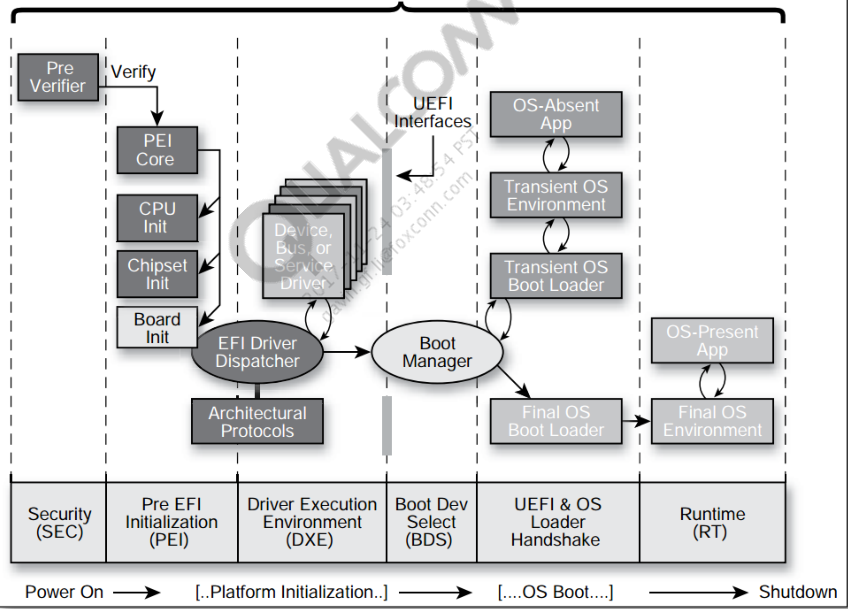
\includegraphics[width=13cm]{img/ueficompon}
\caption{uefi step}
\label{step}
\end{center}
\vspace{-0.5em}
\end{figure}



\begin{figure*}[htbp]
\begin{center}
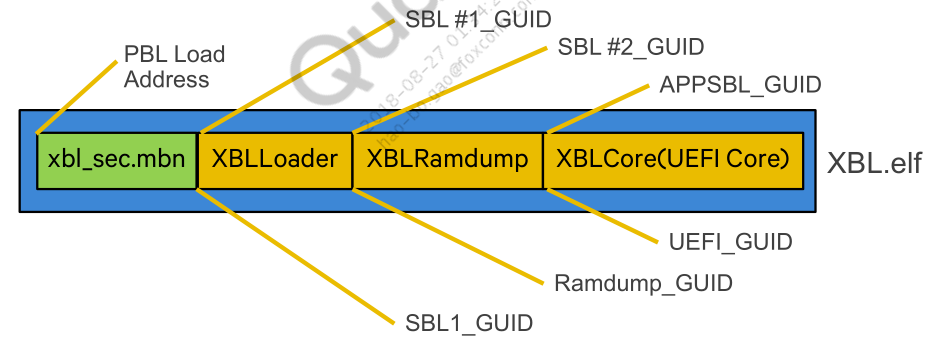
\includegraphics[width=13cm]{img/xbl_reg}
\caption{xbl region}
\label{xblreg}
\end{center}
\vspace{-0.5em}
\end{figure*}


\begin{figure*}[htbp]
\begin{center}
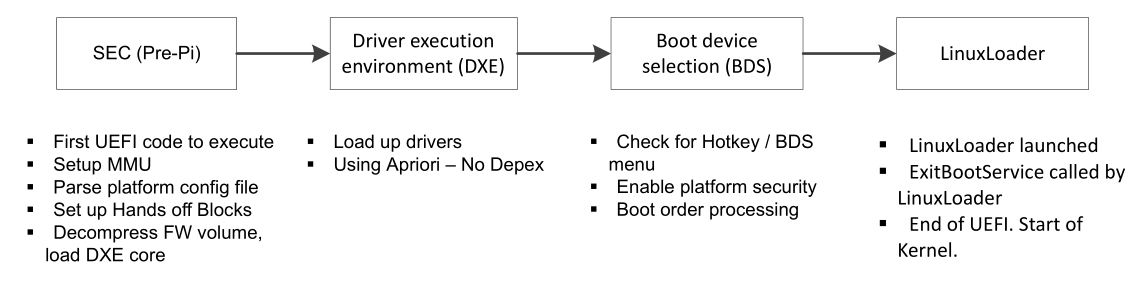
\includegraphics[width=15cm]{img/uefistage}
\caption{uefi 阶段}
\label{xblstage}
\end{center}
\vspace{-0.5em}
\end{figure*}

\section{uefi 入口}

\begin{lstlisting}
S - Boot Config @ 0x00786070 = 0x000001c1

S - JTAG ID @ 0x00786130 = 0x000ac0e1

S - OEM ID @ 0x00786138 = 0x00000000

S - Serial Number @ 0x00784138 = 0xcd2bcd5b

S - OEM Config Row 0 @ 0x00784188 = 0x0000000000000000

S - OEM Config Row 1 @ 0x00784190 = 0x0000000000000000

S - Feature Config Row 0 @ 0x007841a0 = 0x0070302012400300

S - Feature Config Row 1 @ 0x007841a8 = 0x0000000000000820


111struct boot_log_raw_fuse_entry
{
  uint32 fuse_address;
  char * fuse_name;
  boolean full_row;           /* Indicates full 64 bit row should be logged.  Default is 32 bits. */
  boolean secboot_protected;  /* If secboot is enabled then do not log this entry. */
};

static struct boot_log_raw_fuse_entry boot_log_raw_fuse_entries[] =
{
   { BOOT_LOGGER_BOOT_CONFIG_FUSE_ADDRESS, "Boot Config", FALSE, FALSE },
    { BOOT_LOGGER_JTAG_ID_FUSE_ADDRESS, "JTAG ID", FALSE, FALSE },
    { BOOT_LOGGER_OEM_ID_FUSE_ADDRESS, "OEM ID", FALSE, FALSE },
    { BOOT_LOGGER_SERIAL_NUM_FUSE_ADDRESS, "Serial Number", FALSE, FALSE },
    { BOOT_LOGGER_OEM_CONFIG_ROW_0_FUSE_ADDRESS, "OEM Config Row 0", TRUE, TRUE },
    { BOOT_LOGGER_OEM_CONFIG_ROW_1_FUSE_ADDRESS, "OEM Config Row 1", TRUE, TRUE },
    { BOOT_LOGGER_FEATURE_CONFIG_ROW_0_FUSE_ADDRESS, "Feature Config Row 0", TRUE, FALSE },
    { BOOT_LOGGER_FEATURE_CONFIG_ROW_1_FUSE_ADDRESS,"Feature Config Row 1", TRUE, FALSE },
    { 0, NULL, FALSE, FALSE }
};

/PL2P/BOOT.XF.1.4/boot_images/QcomPkg/XBLLoader/boot_logger.c 

由 boot_log_raw_fuse_values 写到bootlog_buffer
snprintf(bootlog_buffer,BOOT_LOG_TEMP_BUFFER_SIZE,"%s @ 0x%08x = 0x%08x",boot_log_raw_fuse_entries[count].fuse_name,
boot_log_raw_fuse_entries[count].fuse_address,*current_fuse);

boot_images/QcomPkg/XBLLoader/ModuleEntryPoint.S 
_ModuleEntryPoint:
 b sbl1_entry

 
 
sbl1_entry:
  MOV w0, w7
  BL sbl1_main_ctl
  
This file bootstraps the processor. The Start-up Primary Bootloader
(SBL1) performs the following functions:

    - Set up the hardware to continue boot process.
    - Initialize DDR memory
    - Load Trust-Zone OS
    - Load RPM firmware
    - Load APPSBL and continue boot process

  

 
  
sbl1_main_ctl -> sbl1_boot_logger_init->boot_log_init->boot_log_raw_fuse_values

boot_config_process_bl(&bl_shared_data,SBL1_IMG,sbl1_config_table);
 

 
 
\boot_images\QcomPkg\Sdm660Pkg\Library\XBLLoaderLib\sbl1_config.c



/**
 * Boot configuration table entry 
 */
typedef struct
{
  image_type host_img_id;                 /**< Image ID of the host */
  config_image_type host_img_type;        /**< Image type of the host */ 
  image_type target_img_id;               /**< Image ID of the target */ 
  config_image_type target_img_type;      /**< Image type of the target */ 
  secboot_sw_type target_img_sec_type;    /**< Secure Software ID of the target */
  boot_boolean load;                      /**< Target will be loaded */
  boot_boolean auth;                      /**< Target will be authenticated */
  boot_boolean exec;                      /**< Target will execute immediately after
                                               loading/authentication */
  boot_boolean jump;                      /**< Target will be jumped to after
                                               post procedures are complete */ 
  boot_procedure_func_type exec_func;     /**< Function pointer to execute function.
                                               Must be defined if exec is TRUE */ 
  boot_procedure_func_type jump_func;     /**< Function pointer to jump function.
                                               Must be defined if jump is TRUE */ 
  boot_procedure_func_type *pre_procs;    /**< Function pointer array to pre-procedures */
  boot_procedure_func_type *post_procs;   /**< Function pointer array to post-procedures */
  boot_logical_func_type boot_load_cancel;/**< Function pointer to cancel loading */ 
  uint8 * target_img_partition_id;        /**< Target image partition ID information */
  uint8 * target_img_str;                  /**< Target image name information  */
  whitelist_region_type * whitelist_table; /**< Whitelist table */
  boot_boolean boot_ssa_enabled;           /**< Subsystem self authentication (ssa)*/
  boot_boolean enable_rollback_protection; /**< Enable Roll back protection feature or not */
  boot_boolean enable_xpu;                 /**< Enable XPU configuration for the image */
  uint32 xpu_proc_id;                      /**< XPU proc id to be passed to TZ */
  uint32 sbl_qsee_interface_index;        /**< Index of this image's entry in sbl qsee interface struct */
  uint64 seg_elf_entry_point;             /**< Entry point for segmented ELF */
  uint32 RESERVED_3;                      /**< RESERVED */
  uint32 RESERVED_4;                      /**< RESERVED */
}boot_configuration_table_entry;


 /*==========================================================================
                      DEFINE TARGET BOOT CONFIG TABLE
===========================================================================*/
boot_configuration_table_entry sbl1_config_table[] = 
{




void boot_config_process_bl(bl_shared_data_type *bl_shared_data,image_type host_img,boot_configuration_table_entry * boot_config_table )
{
  boot_configuration_table_entry *curr_entry = NULL;

  BL_VERIFY( bl_shared_data != NULL && boot_config_table != NULL,
             BL_ERR_NULL_PTR_PASSED|BL_ERROR_GROUP_BOOT);

  /* For every entry in the boot configuration table */
  for(curr_entry = boot_config_table;
      curr_entry->host_img_id != NONE_IMG;
      curr_entry++)
  {
    /* Process entries sequentially only for the specific host_img */
    if(curr_entry->host_img_id == host_img)
    {
      boot_config_process_entry(bl_shared_data,
                                curr_entry);
    }
  }
 
  return;
}

 
\end{lstlisting}









\begin{itemize}

\item 

\item 

\end{itemize}


\section{uefi DXE}


\section{uefi BDS}





\section{uefi LINUX LOADER}




\section{浅谈 linux init}

在start\_kernel 中 内核初始化的最后部分 有对 rest\_init的调用

这个函数的使命就是起init 进程。

start\_kernel -> rest\_init


rest\_init 中 有
\begin{lstlisting}
// 一号进程 
kernel_thread(kernel_init, NULL, CLONE_FS | CLONE_SIGHAND);
// 二号进程 
pid = kernel_thread(kthreadd, NULL, CLONE_FS | CLONE_FILES);

// 0 号进程 
cpu_idle();
\end{lstlisting}
kernel\_init 就是init 进程



kernel\_init -> do\_basic\_setup



